\section{Introduction} \label{sec:environmentIntroduction}
In this chapter the setup of the autonomous vehicle is presented. 
Here all microcontroller which were considered to be used are listed.
Also the main usage of most of them is shown.
Another topic of this chapter is an introduction to the environment of Arduino.
Last but not least the different types which were used in this project of sensors are shown.


\section{AVR} \label{sec:AVR}
Throughout this section all informations and pictures are taken from \cite{web:Atmel}, otherwise it is described separately.

AVR is the name of a microcontroller-family which is produced by the company Atmel.
Atmel currently produces different types of microcontrollers.
These types can be grouped in:

\begin{itemize}
\item 32-bit AVR UC3
\item AVR XMEGA
\item Automotive AVR
\item megaAVR
\item tinyAVR
\end{itemize}

These families differ in size of memory, clock rate and the supply voltage which is needed by the controller.
As an example the tinyAVR also known as ATtiny is a very small and cheap microcontroller which only needs a power supply of 0,7 V.
Beside these listed chips there are other ones which have the function to handle the battery management of Li-Ion batteries.
In addition to AVR Atmel also produces other chip-families.
For details we refer to \url{ http://www.atmel.com/products/microcontrollers/avr/default.aspx }

For this thesis mostly megaAVR also known ATmega are used because these are the most popular ones and so they are used on the Arduino boards.
These boards are shown in \ref{sec:arduino}.


\subsection{ATmega~2560} \label{sec:atmega2560}
In this section all informations and pictures are taken from \cite{manual:atmega2560}.

We start with a brief description of the AVR microcontroller which is used on the Arduino~Mega~2560 boards.
These boards will be shown in \ref{sec:arduino}.
ATmega~2560 is part of many different electronic projects.
It is a very many-sided microcontroller because it has has a lot of different features implemented in hardware.
This chip contains a lot of input and output interfaces so it can communicate with other chips without wasting invaluable computing time.
Another advantage of this these hardware implemented I/O interfaces is that no code has to be written .

In the following the main technical features will be summarized:


\subsubsection{Summary} \label{sec:atmega2560Summary}
\begin{tabular}{ll}
Speed Grade	& 0-16 MHz	\\
Flash Memory	& 256 KB	\\
SRAM			& 8 KB	\\
EEPROM		& 4 KB	\\
I/O Lines		& 86		\\
8-bit Timer		& 2		\\
16-bit Timer	& 4		\\
4-bit PWM		& 4		\\
2 to 16-bit PWM	& 12		\\
10-bit ADC		& 16		\\
USART / UART	& 4		\\
TWI / I2C		& 1		\\
\end{tabular}


\section{Arduino} \label {sec:arduino}
In this section all information and pictures are taken from \cite{web:arduino} otherwise it is described separately.

The term Arduino stands for a full environment to program different microcontrollers.
All parts of the Arduino environment are a open source. 
The environment is offered with different boards which vary in size, features, price, ... .
On each board there is the full hardware to program and run the microcontroller.
So a USB to serial tunneler is installed on-board.
Most boards also contain a voltage regulator to feed it by an external power supply too and a circuit to switch to the USB power supply.
At least each board contain a button to reset the microcontroller.

Another Part of the Arduino environment is the Arduino software.
With this software it is possible to compile C++ code with the avr-gcc compiler which is part of the GNU Compiler Collection.
This software can also transfer the compiled sketch to the USB to serial converter and this chip programs the microcontroller.

A further part of the Arduino environment is the library.
This library contains code to address the pins.
In result of that the sketch code is more compact and therefore easier to read.


\subsection{Arduino Shields} \label{sec:arduinoShields}
Shields are boards which have the design that they can be plugged on top of the Arduino.
Those shields are used to extend the Arduino capabilities.
Most shields are designed for the Arduino~UNO but the design of the Arduino~Mega is compatible for most of the shields of the Arduino~UNO.
But the shields of the Arduino~Mega does not fit on an Arduino~UNO because it has much more pins and functions than the Arduino~UNO.

Examples for Arduino Shields are:
\begin{itemize}
\item MotorDriver Shields
\item GPS Shields
\item Memory Shields
\item Display Schields
\end{itemize}


\subsection{Arduino~Mega~2560} \label {sec:arduinoMega2560}
\begin{figure}
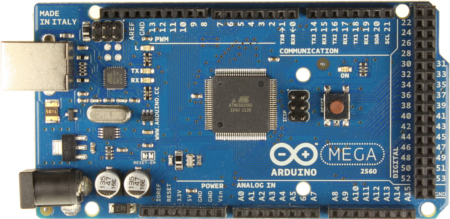
\includegraphics[scale=0.5]{picturesArduino/arduinoMega2560_R3_Front.jpg}
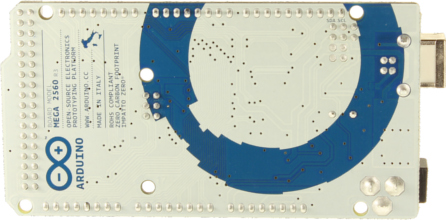
\includegraphics[scale=0.5]{picturesArduino/arduinoMega2560_R3_Back.jpg}
\caption{Board of the Arduino Mega 2560}
\label{fig:mega2560}
\end{figure}

The Arduino~Mega~2560 is a microcontroller board based on the ATmega~2560.
Basically this is a board holding an ATmega~2560 so the technical features from the ATmega~2560 are also applicable for the Arduino~Mega~2560.
See figure~\ref{fig:mega2560} for an image of this microcontroller.
 


\subsection{Datatypes} \label {sec:datatypes}
Here the data types of AVRs are described because they differ significantly from the sizes normally used on ``regular'' PCs.
One example is the type int which only has a size of 2 bytes instead of 4 bytes like on an PC.
Another very interesting type is floating-point numbers. 
On AVRs floating-point calculations have some significant characteristics.
A very interesting fact is that floating-point calculations are much slower than integer calculations in relation to regular CPUs because AVRs have no floating point unit.
This means that floating-point calculations have to be emulated by other operations. Also the precision of floating-point calculations differs from usual PCs.
On a PC a float has a size of 4 bytes and a double has a size of 8 bytes.
On AVRs a double is as large as a float and has 4 bytes. As a consequence the usual precision is six to seven digits.
See table~\ref{tab:datatypes} for details.

\begin{table}
{\large
\begin{center}
\begin{tabular}{|l|r|r|r|}
\hline
\multirow{2}{*}{data type} & \multirow{2}{*}{Bit} & \multicolumn{2}{|c|}{value}  \\
\cline{3-4}
& & min & max \\
\hline
int8\_t, signed char				& $8$	& $-2^{7}$		& $2^{7}-1$	\\
int16\_t, signed short, signed int		& $16$	& $-2^{15}$		& $2^{15}-1$	\\
int32\_t, signed long				& $32$ 	& $-2^{31}$		& $2^{31}-1$	\\
int64\_t, signed long long			& $64$ 	& $-2^{63}$		& $2^{63}-1$	\\
& & & \\
uint8\_t, unsigned char			& $8$	& $0$			& $2^{8}-1$	\\
uint16\_t, unsigned short, unsigned int	& $16$ 	& $0$ 			& $2^{16}-1$	\\
uint32\_t, unsigned long			& $32$ 	& $0$			& $2^{32}-1$	\\
uint64\_t, unsigned long long		& $64$ 	& $0$			& $2^{64}-1$	\\
& & & \\
float, double					& $32$ 	& $-3.4028235*10^{38}$	& $3.4028235*10^{38}$	\\
\hline
\end{tabular}
\end{center}
}
\caption{Sizes of data types on the AVR}
\label{tab:datatypes}
\end{table}



\subsection{Microcontroller I/O} \label{sec:microcontrollerIO}
In this section the interface to the Arduino I/O is described.
First the basic analog and digital I/O is shown.
This is followed by a description of the UART API. 
Finally the I2C is described.
For the more complex parts of the I/O we give small code snippets to illustrate the programming of the I/O!


\subsubsection{Input Pins:} \label{sec:inputPins}
The following instruction describes how a value can be read from a pin.
\begin{itemize}
\item First the pin has to be brought into input mode.\\
\lstinline|pinMode(pin, INPUT);|

\item Then the internal pull up resistor can either be switched on or off.\\
Turn on:\\
\lstinline|digitalWrite(pin, HIGH);|\\
Turn off:\\
\lstinline|digitalWrite(pin, LOW);|\\

\item If the microcontroller has the right settings the pin can be read.
One possibility is to read a digital value.
This returns False if the voltage is lower than 2 volts and True if the voltage is above 3 volts.
If the voltage is between 2 and 3 volts either True or False can be returned.
In this case the result can be random.\\
\lstinline|value = digitalRead(pin);|\\
The other possibility is to read an analog value.
This returns a value with a resolution of 10 Bit.
So it will return a value between 0 and 1024.
0 stand for 0V and 1024 stand for 5V.\\
\lstinline|value = analogRead(Apin)|\\
\end{itemize}


\subsubsection{Digital Output Pins}\label{sec:digitalOutputPins}
The digital output of the Arduino ports can be used to send data or switch some components off and on.
Very interesting is that the the high output voltage is lower than the supply voltage and the low output voltage is higher than the supply voltage.
This is because the transistors inside the IC have a small voltage drop.
Before the digital output pins can be used the pinmode has to be set to output:\\
\lstinline|pinMode(pin, OUTPUT);|\\
To write a low voltage on the port this code line have to be executed:\\
\lstinline|digitalWrite(pin, LOW);|\\
This code line write a high voltage on the port:\\
\lstinline|digitalWrite(pin, HIGH);|\\


\subsubsection{Analog Output Pins - PWM}\label{sec:analogOutputPinsPWM}
\begin{figure}
\tikzstyle{line}=[color=black,line width=1.5pt]
\newcommand*{\drawPWMschematic}[1]{
	\pgfmathsetmacro{\value}{#1 / 255}
	\pgfmathtruncatemacro{\dutyCycle}{round(100 * \value)}
	\draw(3,1) node[above]{\makebox[0pt][l]{\dutyCycle\%~Duty Cycle - analogWrite(#1)} };
	\draw(-0.5,1) node[left]{\makebox[0pt][l]{5V} };
	\draw(-0.5,0) node[left]{\makebox[0pt][l]{0V} };
	\pgfmathsetmacro{\offValue}{1 - \value}	
	\drawSquarewave{line}{5}{\value}{\offValue}{2}{1}
}
\makebox[\linewidth]{
\begin{tikzpicture}
	\newcounter{cpos}
	\foreach \n in {0,64,127,191,255} {
		\pgfmathsetmacro{\pos}{\value{cpos} * 1.65}
		\begin{scope}[shift={(0,\pos )}]
			\drawPWMschematic{\n}
		\end{scope}
		\stepcounter{cpos}
        }
\end{tikzpicture}
}
\caption{Schematic of PWM}
\label{fig:pwm}
\end{figure}

PWM, which stand for pulse width modulation, is one of many methods to produce an analog voltage.
The main thing to know that PWM in the strict sense doesn't make a real analog voltage.
In truth PWM switches the pin frequently on and off. 
Many electronic components allow to give the required input via PWM.
If a real analog signal is required smoothing capacitors can be used.
This capacitors work as low pass filter and return a real analog voltage.
For an illustration of PWM see figure~\ref{fig:pwm}. 
Example for electronic components which can be controlled with PWM and their usage are:
\begin{itemize}
\item Led
	\subitem Car's brake light
	\subitem Background lighting of displays
\item Motor driver
	\subitem CPU air cooler
	\subitem Speed control of model cars
\item Servo
	\subitem Steering control of model cars
	\subitem Arms of industrial robots
\item Smoothing capacitors
	\subitem Data transfer
	\subitem Reference voltage for sensors

\end{itemize}

The resolution of the PWM pins are 8 bit so the minimal value is 0 which equals to the low level voltage and the maximal value is 255 which equals to the high level voltage. 
To output a PWM signal the port has to be set as output. 
A general description can be found in the section~\ref{sec:digitalOutputPins}.
Then the following code line can be executed.\\
\lstinline|analogWrite(PWMpin, value);|



\subsubsection{UART}\label{sec:uart}
The term UART means Universal Asynchronous Receiver Transmitter also known as RS-232.
UART is a serial interface and was one of the most important interfaces on PCs until it got replaced by USB. On microcontrollers it still plays an important role nowadays.
To use the RS-232 interface on newer PCs it is possible to tunnel it trough USB or Bluetooth. 
The OS of the PC creates a virtual RS-232 interface.
To create a tunnel of a RS-232 interface above USB it is possible to use an IC which provides such functionality.
Another possibility is to completely emulate the RS-232 tunnel via software.
This is also the method which is used on the Arduino.

To use the UART on the Arduino the following code has to be executed.\\
Before the serial connection is used it has to be started: \\
\lstinline|Serial.beginn(speed);| \\
Then data which have a size of one byte can be written to the serial port.
If there is more than one byte this method has to be called for each byte: \\
\lstinline|Serial.write(value);| \\
Or something can be printed to the serial port. 
This can be used instead of Serial.write:\\
\lstinline|Serial.println(value);| \\

A small code snippet for a serial connection could look like this:\\
\begin{lstlisting}
Serial.begin(9600);
Serial.println("Hello World");
byte in;
while(Serial.available() > 0)
	in = Serial.read();
char c = Serial.read();
\end{lstlisting}



\subsubsection{I2C}\label{sec:i2c}
The I2C bus is also a serial bus like UART with the difference that I2C uses a master and slave administration.
Another difference is, that more then two devices can be joined to the I2C bus.
The address has 7 bits and so it can be set from 0 to 127.
This result in a maximal number of devices of 128.

To use the I2C bus on the Arduino the following code has to be executed.\\
At first the I2C bus has to be started: \\
\lstinline|Wire.beginn(address);| \\
Then a request can be started: \\
\lstinline|Wire.requestFrom(device,size);| \\
At least one byte can be read from the device.
If the manual of the device say that there is more than one byte this method can be executed more than once. \\
\lstinline|byte b = Wire.read();| \\
Another option is to start a transmission:\
\lstinline|Wire.beginTransmission(device);| \\
Then it is possible to write data to the communication partner:\\
\lstinline|Wire.write(value);|\\
After sending the data the transmmission have to be closed:\\
\lstinline|Wire.endTransmission();|\\
An example for an I2C connection could look like this:\\
\begin{lstlisting}
Wire.begin()
Wire.requestFrom(0x23,1);
byte b = Wire.read();
Wire.beginTransmission(0x23);
Wire.write(b);
Wire.endTransmission();
\end{lstlisting}


\section{Electronic Components and Circuits}\label{sec:electronicCircuits}
This section contains explanations to different electronic components and circuits which were used during this thesis.


\subsection{Operational Amplifier}\label{sec:operationalAmplifier}

\newcommand\opampfive[5]
{
\begin{circuitikz}
\draw (0,0) node[op amp] (opamp) {};
\draw (-2,-0.49) to[short, o-] (opamp.+) (-2.2,-0.49) node[anchor=east] {${#1}$};
\draw (-2,0.49) to[short, o-] (opamp.-) (-2.2,0.49) node[anchor=east] {${#2}$};
\draw (-0.08,1.5) to[short, o-] (opamp.up) (-0.08,1.6) node[anchor=south] {${#3}$};
\draw (-0.08,-1.5) to[short, o-] (opamp.down) (-0.08,-1.6) node[anchor=north] {${#5}$};
\draw (1,0) to[short, -o] (2,0) -- (opamp.out) (2.1,0) node[anchor=west] {${#4}$};
\end{circuitikz}
}

\begin{figure}
\center
\begin{circuitikz}
\draw (0,0) node[op amp] (opamp) {};
\draw (-2,-0.49) to[short, o-] (opamp.+) (-2.2,-0.49) node[anchor=east] {Vin+};
\draw (-2,0.49) to[short, o-] (opamp.-) (-2.2,0.49) node[anchor=east] {Vin-};
\draw (-0.08,1.5) to[short, o-] (opamp.up) (-0.08,1.6) node[anchor=south] {+};
\draw (-0.08,-1.5) to[short, o-] (opamp.down) (-0.08,-1.6) node[anchor=north] {-};
\draw (1,0) to[short, -o] (2,0) -- (opamp.out) (2.1,0) node[anchor=west] {out};
\end{circuitikz}
\caption{Operational Amplifier Schematic}
\label{fig:operationalAmplifier}
\end{figure}


\subsection{Amplifier}\label{sec:Amplifier}
Some possibilities to amplify are:
\begin{itemize}
\item Transistors
\item FETs
\item Operation Amplifier
\item Amplifier circuit based on an operation amplifier
\item ...
\end{itemize}
The result of the used amplifier can be different.\\
At the most sensor it can be measured both the current and voltage but most sensors have one property which is easier to measure.


\subsection{Schmitt Trigger}\label{sec:schmittTrigger}
A Schmitt Trigger is a important electronic part.
It can be used as an antibeat device or relaxation oscillator.
In this diploma thesis it is only used as an antibeat device.
One application for an Schmitt Trigger is to transform the signal of an rotary encoder which is similar to a sinus wave to an clear binary signal.
A Schmitt Trigger can be build with an resistor network to an operating amplifier.
The schematic is shown in figure~\ref{fig:schmittTriggerSchematic}.
Schmitt-triggers with a constant hysteresis can also be bought as an IC.
The hysteresis is the voltage difference between the voltage which is needed to set the Schmitt Trigger's output to high and the voltage which is needed to set the Schmitt Trigger's output to low.
For an illustration see figure~\ref{fig:schmittTriggerInputOutputDiagram}.

\begin{figure}
\center
\begin{circuitikz}
\draw (0,0) node[op amp] (opamp) {};
\draw (-4,-0.49) node[anchor=east]{In} to[resistor,o-] (-2,-0.49) -- (opamp.+) (-2.2,-0.49);
\draw (-1.5,-0.49) -- (-1.5, -2) to[resistor] (1.5,-2) -- (1.5,0);
\draw (-2,0.49) node[anchor=east]{Gnd} to[short, o-] (opamp.-) (-2.2,0.49);
\draw (1,0) to[short, -o] (2,0) -- (opamp.out) (2.1,0) node[anchor=west] {Out};
\end{circuitikz}
\caption{Inverting Schmitt Trigger Schematic}
\label{fig:schmittTriggerSchematic}
\end{figure}

\begin{figure}
\pgfmathsetmacro{\pos}{0.2}
\pgfmathsetmacro{\sinFactor}{0.2}
\begin{tikzpicture}
	\begin{scope}[xscale=3, yscale=3]
	 	%Draw grid
		%\draw [color=gray!50]  [step=1] (0,0) grid (15,3);
		%Draw axles
		\draw[->,thick] (0,0) -- (5,0) node[right] {$x$};
		\draw[->,thick] (0,0) -- (0,1.5) node[above] {$y$};
		\draw (0,0)[color=green,line width=1.5pt] plot [const plot] coordinates{(0,0) (0+\pos,0) (0+\pos,1) (1+\pos,1) (1+\pos,0) (2+\pos,0) (2+\pos,1) (3+\pos,1) (3+\pos,0) (4+\pos,0) (4+\pos,1) (4.5,1)};
		%Draw Sin
		\draw (0,0)[color=blue] plot[domain=0:4.5,samples=200] (\x ,{ sin(\x*pi*115 / 2) / 2+0.5 });
		\draw(0,0)[-,thick,color=red] (0,{sin(\pos*pi*115 / 2) / 2+0.5}) --+(4.5,0);
		\draw(0,0)[-,thick,color=red] (0,{-sin(\pos*pi*115 / 2) / 2+0.5}) --+(4.5,0);
		%\draw[gray,->] (-0.3,0) -- (pi+0.3,0);
	\end{scope}
\end{tikzpicture}
\caption{Schmitt Trigger Input Output Diagram}
\label{fig:schmittTriggerInputOutputDiagram}
\end{figure}


\subsection{H-Bridge}\label{sec:hBridge}
This electronic circuit is used to control a motor.
The main advantage against a usual MOSFET or Transistor is that the H-bridge can swap the direction of the motor power supply and so it is possible to let the motor turn backward.
A H-bridge consists of four relays, transistors or MOSFETs.
The detailed circuit is shown in Figure~\ref{fig:hbridgeSchematic}.
H-bridges can be bought in a single IC with different interfaces and different allowed power.

A example for an H-bridge IC is the TB6612FNG.
This IC can handle two different motors.
The interface of this IC consists of three pins for each motor and one general power down pin.
From the three pins are two pins which control if the motor is on forward, on backward, off or like a brake.
The third pin control the speed of the motor.
The input signal of this pin have to be a PWM signal.

\begin{figure}
\makebox[\textwidth][c]{
\begin{circuitikz}
\draw
(0,0) to[battery,l=$V_{\text{}}$] ++(0,4)
++(0,0) -- ++(2,0) coordinate (LT)
%%%  H-bridge 1st leg
(LT) ++(2,-1) node [npn,scale=1,name=igbt1] {}
++(0,-2) node [npn,scale=1,name=igbt3] {}
(igbt1.C) |- (LT)
(igbt1.E) -- (igbt3.C)
(igbt3.E) |- (0,0)
%%% H-bridge 2nd leg
(LT) ++(4,-1) node [npn,scale=1,name=igbt2] {}
++(0,-2) node [npn,scale=1,name=igbt4] {}
(igbt2.C) |- (LT)
(igbt2.E) -- (igbt4.C)
(igbt4.E) |- (0,0)
%%% Output
(igbt1.E) node[circ] {} to[short,-o] ++(3,0) node[anchor=west] {Ma}
(igbt4.C) node[circ] {} to[short,-o] ++(1,0) node[anchor=west] {Mb}
%%% Motor Control
(2,-0.5) rectangle (6,-1.5)
(3,-0.5) |- (igbt1.B)
(3.2,-0.5) |- (igbt3.B)
(5,-0.5) |- (igbt2.B)
(5.2,-0.5) |- (igbt4.B)
;
\node (note1) at (4,-1) {Motor Control};
\end{circuitikz}

}
\caption{H-Bridge Schematic}
\label{fig:hbridgeSchematic}
\end{figure}



\section{Mathematic Algorithms}\label{sec:mathematicAlgorithms}


\subsection{Regression}\label{sec:regression}


